
\documentclass[10pt,twocolumn,letterpaper]{article}

\usepackage{iccv}
\usepackage{times}
\usepackage{epsfig}
\usepackage{graphicx}
\usepackage{amsmath}
\usepackage{amssymb}
\usepackage[numbers,sort]{natbib}

\usepackage{subfigure}
\usepackage{upgreek}
\usepackage{multirow}
\usepackage{color}
\usepackage{bm}
\DeclareMathOperator*{\argmin}{arg\,min}
\usepackage{arydshln}
\usepackage{latexsym}


\usepackage{amsthm}
\newtheorem{theorem}{Theorem}
\newtheorem{lemma}[theorem]{Lemma}
\newtheorem{conj}[theorem]{Conjecture}


% Include other packages here, before hyperref.

% If you comment hyperref and then uncomment it, you should delete
% egpaper.aux before re-running latex.  (Or just hit 'q' on the first latex
% run, let it finish, and you should be clear).
\usepackage[pagebackref=true,breaklinks=true,letterpaper=true,colorlinks,bookmarks=false]{hyperref}

% \iccvfinalcopy % *** Uncomment this line for the final submission

\def\iccvPaperID{572} % *** Enter the ICCV Paper ID here
\def\httilde{\mbox{\tt\raisebox{-.5ex}{\symbol{126}}}}

% Pages are numbered in submission mode, and unnumbered in camera-ready
\ificcvfinal\pagestyle{empty}\fi
\begin{document}

%%%%%%%%% TITLE
\title{Supplementary File to ``Multi-channel Weighted Nuclear Norm Minimization for Real Color Image Denoising''}

\author{First Author\\
Institution1\\
Institution1 address\\
{\tt\small firstauthor@i1.org}
% For a paper whose authors are all at the same institution,
% omit the following lines up until the closing ``}''.
% Additional authors and addresses can be added with ``\and'',
% just like the second author.
% To save space, use either the email address or home page, not both
\and
Second Author\\
Institution2\\
First line of institution2 address\\
{\tt\small secondauthor@i2.org}
}

\maketitle
%\thispagestyle{empty}


\section{Proof of Theorem 1.}
\begin{theorem}
Assume the weights in $\bm{w}$ are in a non-descending order, the sequence $\{\mathbf{X}_{k}\}$, $\{\mathbf{Z}_{k}\}$, and $\{\mathbf{A}_{k}\}$ generated in Algorithm 1 satisfy:
\begin{align}
&(1) \lim_{k \to \infty} \|\mathbf{X}_{k+1}-\mathbf{Z}_{k+1}\|_{F}=0;
\\
&(2) \lim_{k \to \infty} \|\mathbf{X}_{k+1}-\mathbf{X}_{k}\|_{F}=0;
\\
&(3) \lim_{k \to \infty} \|\mathbf{Z}_{k+1}-\mathbf{Z}_{k}\|_{F}=0.
\end{align}
\end{theorem}
\begin{proof}
1.\ Firstly, we proof that the sequence $\{\mathbf{A}_{k}\}$ generated by Algorithm 1 is upper bounded.
Let $\mathbf{X}_{k+1}+\rho_{k}^{-1}\mathbf{A}_{k}
=
\mathbf{U}_{k}\mathbf{\Sigma}_{k}\mathbf{V}_{k}^{\top}$
be its SVD in the $(k+1)$-th iteration. According to Corollary 1 of \cite{wnnmijcv}, we can have the SVD of $\mathbf{Z}_{k+1}$ as $\mathbf{Z}_{k+1}=\mathbf{U}_{k}\hat{\mathbf{\Sigma}}_{k}\mathbf{V}_{k}^{\top}=\mathbf{U}_{k}\mathcal{S}_{\frac{\bm{w}}{\rho_{k}}}(\mathbf{\Sigma}_{k})\mathbf{V}_{k}^{\top}$. 
Then we have 
\begin{align}
\|
\mathbf{A}_{k+1}
\|_{F}
&
=
\|
\mathbf{A}_{k}
+
\rho_{k}
(\mathbf{X}_{k+1}-\mathbf{Z}_{k+1})
\|_{F}
\\
&
=
\rho_{k}\|
\rho_{k}^{-1}
\mathbf{A}_{k}
+
\mathbf{X}_{k+1}
-
\mathbf{Z}_{k+1}
\|_{F}
\\
&
=
\rho_{k}\|
\mathbf{U}_{k}\mathbf{\Sigma}_{k}\mathbf{V}_{k}^{\top}
-
\mathbf{U}_{k}\mathcal{S}_{\frac{\bm{w}}{\rho_{k}}}(\mathbf{\Sigma}_{k})\mathbf{V}_{k}^{\top}
\|_{F}
\\
&
=
\rho_{k}\|
\mathbf{\Sigma}_{k}
-
\mathcal{S}_{\frac{\bm{w}}{\rho_{k}}}(\mathbf{\Sigma}_{k})
\|_{F}
\\
&
=
\rho_{k}
\sqrt{\sum_{i}(\mathbf{\Sigma}_{k}^{ii}-\mathcal{S}_{\frac{w_{i}}{\rho_{k}}}(\mathbf{\Sigma}_{k}^{ii}))^{2}}
\\
&
\le
\rho_{k}
\sqrt{\sum_{i}(\frac{w_{i}}{\rho_{k}})^{2}}
=
\sqrt{\sum_{i}w_{i}^{2}}.
\end{align}
The inequality above can be proofed as follows: given the diagonal matrix $\mathbf{\Sigma}_{k}$, we define $\mathbf{\Sigma}_{k}^{ii}$ as the $i$-th element of $\mathbf{\Sigma}_{k}^{ii}$. If $\mathbf{\Sigma}_{k}^{ii}\ge\frac{w_{i}}{\rho_{k}}$, we have $\mathcal{S}_{\frac{w_{i}}{\rho_{k}}}(\mathbf{\Sigma}_{k}^{ii})=\mathbf{\Sigma}_{k}^{ii}-\frac{w_{i}}{\rho_{k}}\ge 0$. If $\mathbf{\Sigma}_{k}^{ii}<\frac{w_{i}}{\rho_{k}}$, we have $\mathcal{S}_{\frac{w_{i}}{\rho_{k}}}(\mathbf{\Sigma}_{k}^{ii})=0<\mathbf{\Sigma}_{k}^{ii}+\frac{w_{i}}{\rho_{k}}$. After all, we have $|\mathbf{\Sigma}_{k}^{ii}-\mathcal{S}_{\frac{w_{i}}{\rho_{k}}}(\mathbf{\Sigma}_{k}^{ii})|\le\frac{w_{i}}{\rho_{k}}$ and hence the inequality holds true. Hence, the sequence $\{\mathbf{A}_{k}\}$ is upper bounded.

2.\ Secondly, we proof that the sequence of Lagrangian function $\{\mathcal{L}(\mathbf{X}_{k+1},\mathbf{Z}_{k+1},\mathbf{A}_{k},\rho_{k})\}$ is also upper bounded. Since the global optimal solution of $\mathbf{X}$ and $\mathbf{Z}$ in corresponding subproblems, we always have 
$
\mathcal{L}(\mathbf{X}_{k+1},\mathbf{Z}_{k+1},\mathbf{A}_{k},\rho_{k})
\le
\mathcal{L}(\mathbf{X}_{k},\mathbf{Z}_{k},\mathbf{A}_{k},\rho_{k}).
$
Based on the updating rule that 
$
\mathbf{A}_{k+1}
=
\mathbf{A}_{k} + \rho_{k}(\mathbf{X}_{k+1}-\mathbf{Z}_{k+1})
$,
we have 
$
\mathcal{L}(\mathbf{X}_{k+1},\mathbf{Z}_{k+1},\mathbf{A}_{k+1},\rho_{k+1})
=
\mathcal{L}(\mathbf{X}_{k+1},\mathbf{Z}_{k+1},\mathbf{A}_{k},\rho_{k})
+
\langle
\mathbf{A}_{k+1}
-
\mathbf{A}_{k}
,
\mathbf{X}_{k+1}
-
\mathbf{Z}_{k+1}
\rangle
+
\frac{\rho_{k+1}-\rho_{k}}{2}
\|
\mathbf{X}_{k+1}-\mathbf{Z}_{k+1}
\|_{F}^{2}
=
\mathcal{L}(\mathbf{X}_{k+1},\mathbf{Z}_{k+1},\mathbf{A}_{k},\rho_{k})
+
\frac{\rho_{k+1}+\rho_{k}}{2\rho_{k}^{2}}
\|
\mathbf{A}_{k+1}
-
\mathbf{A}_{k}
\|_{F}^{2}
$.
Since the sequence 
$\{\|
\mathbf{A}_{k}\}$
is upper bounded, the sequence 
$\{\|
\mathbf{A}_{k+1}
-
\mathbf{A}_{k}
\|_{F}\}$ is also upper bounded. Denote by $a$ the upper bound of 
$\{\|
\mathbf{A}_{k+1}
-
\mathbf{A}_{k}
\|_{F}\}$, 
we have 
$
\mathcal{L}(\mathbf{X}_{k+1},\mathbf{Z}_{k+1},\mathbf{A}_{k+1},\rho_{k+1})
\le
\mathcal{L}(\mathbf{X}_{1},\mathbf{Z}_{1},\mathbf{A}_{0},\rho_{0})
+
a\sum_{k=0}^{\infty}\frac{\rho_{k+1}+\rho_{k}}{2\rho_{k}^{2}}
=
\mathcal{L}(\mathbf{X}_{1},\mathbf{Z}_{1},\mathbf{A}_{0},\rho_{0})
+
a\sum_{k=0}^{\infty}\frac{\mu+1}{2\mu^{k}\rho_{0}}
\le
\mathcal{L}(\mathbf{X}_{1},\mathbf{Z}_{1},\mathbf{A}_{0},\rho_{0})
+
\frac{a}{\rho_{0}}\sum_{k=0}^{\infty}\frac{1}{\mu^{k-1}}.
$
The last inequality holds since $\mu+1<2\mu$. Since $\sum_{k=0}^{\infty}\frac{1}{\mu^{k-1}}<\infty$, the sequence of Lagrangian function 
$\mathcal{L}(\mathbf{X}_{k+1},\mathbf{Z}_{k+1},\mathbf{A}_{k+1},\rho_{k+1})$
is upper bound.

3. Thirdly, we proof that the sequences of 
$\{\mathbf{X}_{k}\}$ and $\{\mathbf{Z}_{k}\}$ are upper bounded. Since 
$\|\mathbf{W}(\mathbf{Y}-\mathbf{X})\|_{F}^{2}
+
\|\mathbf{Z}\|_{\bm{w},*}
=
\mathcal{L}(\mathbf{X}_{k},\mathbf{Z}_{k},\mathbf{A}_{k-1},\rho_{k-1})
-
\langle
\mathbf{A}_{k},
\mathbf{X}_{k}-\mathbf{Z}_{k}
\rangle
-
\frac{\rho_{k}}{2}
\|
\mathbf{X}_{k}-\mathbf{Z}_{k}
\|_{F}^{2}
=
\mathcal{L}(\mathbf{X}_{k},\mathbf{Z}_{k},\mathbf{A}_{k-1},\rho_{k-1})
+
\frac{1}{2\rho_{k}}
(
\|
\mathbf{A}_{k-1}
\|_{F}^{2}
-
\|
\mathbf{A}_{k}
\|_{F}^{2}
)
$.
Thus $\{\mathbf{W}(\mathbf{Y}-\mathbf{X}_{k})\}$ and $\{\mathbf{Z}_{k}\}$ are upper bounded, and hence
the sequence $\{\mathbf{X}_{k}\}$ is bounded by Cauchy-Schwarz inequality and triangle inequality.
We can obtain that 
$
\lim_{k \to \infty} 
\|\mathbf{X}_{k+1}-\mathbf{Z}_{k+1}\|_{F}
=
\lim_{k \to \infty} 
\rho_{k}^{-1}
\|
\mathbf{A}_{k+1}
-
\mathbf{A}_{k}
\|_{F}
=
0
$ and the equation (1) is proofed.

4. Then we can proof that 
$
\lim_{k \to \infty} 
\|
\mathbf{X}_{k+1}
-
\mathbf{X}_{k}
\|_{F}
=
\lim_{k \to \infty} 
\|
(\mathbf{W}^{\top}\mathbf{W}
+
\frac{\rho_{k}}{2}
\mathbf{I})^{-1}
(\mathbf{W}^{\top}\mathbf{W}\mathbf{Y}
-
\mathbf{W}^{\top}\mathbf{W}\mathbf{Z}_{k}
-
\frac{1}{2}
\mathbf{A}_{k})
-
\rho_{k}^{-1}
(\mathbf{A}_{k}-\mathbf{A}_{k-1})
\|_{F}
\le
\lim_{k \to \infty} 
\|
(\mathbf{W}^{\top}\mathbf{W}
+
\frac{\rho_{k}}{2}
\mathbf{I})^{-1}
(\mathbf{W}^{\top}\mathbf{W}\mathbf{Y}
-
\mathbf{W}^{\top}\mathbf{W}\mathbf{Z}_{k}
-
\frac{1}{2}
\mathbf{A}_{k})
\|_{F}
+
\rho_{k}^{-1}\|
\mathbf{A}_{k}-\mathbf{A}_{k-1}
\|_{F}
=
0
$
and hence (2) is proofed. 

5. Then (3) can be proofed by checking that 
$
\lim_{k \to \infty} 
\|
\mathbf{Z}_{k+1}-\mathbf{Z}_{k}
\|_{F}
=
\lim_{k \to \infty} 
\|
\mathbf{X}_{k}+\rho_{k}^{-1}\mathbf{A}_{k-1}-\mathbf{Z}_{k}
+
\mathbf{X}_{k+1}-\mathbf{X}_{k}
+
\rho_{k}^{-1}
\mathbf{A}_{k-1}
+
\rho_{k}^{-1}
\mathbf{A}_{k}
-
\rho_{k}^{-1}
\mathbf{A}_{k+1}
\|_{F}
\le
\lim_{k \to \infty} 
\|
\mathbf{\Sigma}_{k-1}-\mathcal{S}_{\bm{w}/\rho_{k-1}}(\mathbf{\Sigma}_{k-1})
\|_{F}
+
\|
\mathbf{X}_{k+1}-\mathbf{X}_{k}
\|_{F}
+
\rho_{k}^{-1}
\|
\mathbf{A}_{k-1}
+
\mathbf{A}_{k+1}
-
\mathbf{A}_{k}
\|_{F}
=
0
$
,
where $\mathbf{U}_{k-1}\mathbf{\Sigma}_{k-1}\mathbf{V}_{k-1}^{\top}$ is the SVD of the matrix $\mathbf{X}_{k}+\rho_{k-1}\mathbf{A}_{k-1}$
.
\end{proof}

\begin{figure}
\centering
\subfigure{
\begin{minipage}{0.075\textwidth}
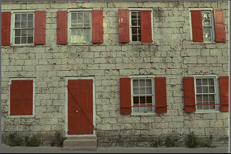
\includegraphics[width=1\textwidth]{24images/resize_kodim01.png}
\end{minipage}
\begin{minipage}{0.075\textwidth}
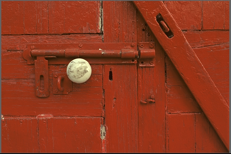
\includegraphics[width=1\textwidth]{24images/resize_kodim02.png}
\end{minipage}
\begin{minipage}{0.075\textwidth}
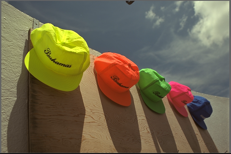
\includegraphics[width=1\textwidth]{24images/resize_kodim03.png}
\end{minipage}
\begin{minipage}{0.075\textwidth}
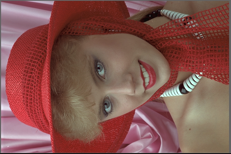
\includegraphics[width=1\textwidth]{24images/resize_kodim04.png}
\end{minipage}
\begin{minipage}{0.075\textwidth}
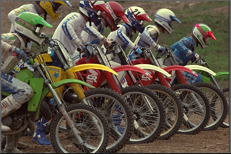
\includegraphics[width=1\textwidth]{24images/resize_kodim05.png}
\end{minipage}
\begin{minipage}{0.075\textwidth}
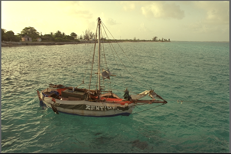
\includegraphics[width=1\textwidth]{24images/resize_kodim06.png}
\end{minipage}
}\vspace{-3mm}
\subfigure{
\begin{minipage}{0.075\textwidth}
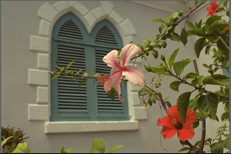
\includegraphics[width=1\textwidth]{24images/resize_kodim07.png}
\end{minipage}
\begin{minipage}{0.075\textwidth}
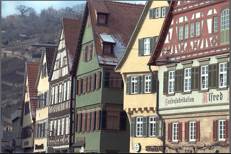
\includegraphics[width=1\textwidth]{24images/resize_kodim08.png}
\end{minipage}
\begin{minipage}{0.075\textwidth}
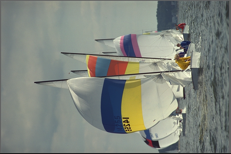
\includegraphics[width=1\textwidth]{24images/resize_kodim09.png}
\end{minipage}
\begin{minipage}{0.075\textwidth}
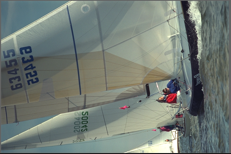
\includegraphics[width=1\textwidth]{24images/resize_kodim10.png}
\end{minipage}
\begin{minipage}{0.075\textwidth}
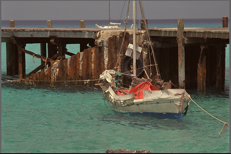
\includegraphics[width=1\textwidth]{24images/resize_kodim11.png}
\end{minipage}
\begin{minipage}{0.075\textwidth}
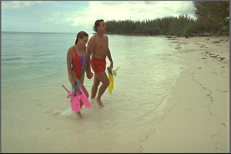
\includegraphics[width=1\textwidth]{24images/resize_kodim12.png}
\end{minipage}
}\vspace{-3mm}
\subfigure{
\begin{minipage}{0.075\textwidth}
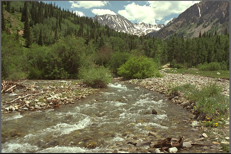
\includegraphics[width=1\textwidth]{24images/resize_kodim13.png}
\end{minipage}
\begin{minipage}{0.075\textwidth}
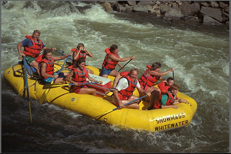
\includegraphics[width=1\textwidth]{24images/resize_kodim14.png}
\end{minipage}
\begin{minipage}{0.075\textwidth}
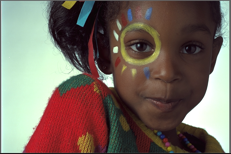
\includegraphics[width=1\textwidth]{24images/resize_kodim15.png}
\end{minipage}
\begin{minipage}{0.075\textwidth}
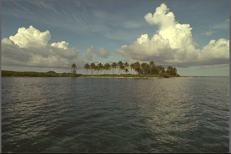
\includegraphics[width=1\textwidth]{24images/resize_kodim16.png}
\end{minipage}
\begin{minipage}{0.075\textwidth}
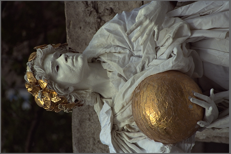
\includegraphics[width=1\textwidth]{24images/resize_kodim17.png}
\end{minipage}
\begin{minipage}{0.075\textwidth}
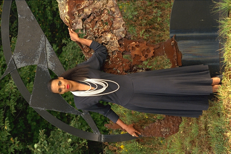
\includegraphics[width=1\textwidth]{24images/resize_kodim18.png}
\end{minipage}
}\vspace{-3mm}
\subfigure{
\begin{minipage}{0.075\textwidth}
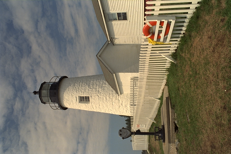
\includegraphics[width=1\textwidth]{24images/resize_kodim19.png}
\end{minipage}
\begin{minipage}{0.075\textwidth}
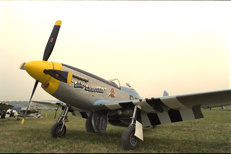
\includegraphics[width=1\textwidth]{24images/resize_kodim20.png}
\end{minipage}
\begin{minipage}{0.075\textwidth}
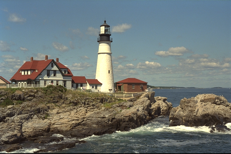
\includegraphics[width=1\textwidth]{24images/resize_kodim21.png}
\end{minipage}
\begin{minipage}{0.075\textwidth}
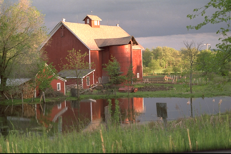
\includegraphics[width=1\textwidth]{24images/resize_kodim22.png}
\end{minipage}
\begin{minipage}{0.075\textwidth}
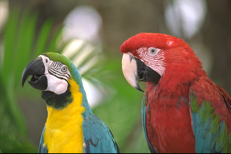
\includegraphics[width=1\textwidth]{24images/resize_kodim23.png}
\end{minipage}
\begin{minipage}{0.075\textwidth}
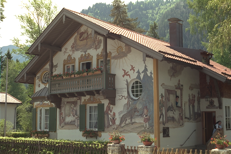
\includegraphics[width=1\textwidth]{24images/resize_kodim24.png}
\end{minipage}
}\vspace{1mm}
\caption{The 24 high quality color images from the Kodak PhotoCD Dataset.}
\label{f2}
\vspace{-2mm}
\end{figure}

Fig.\ \ref{f3} shows a scene denoised by the compared methods.\ We can see that the methods of CBM3D and NC would remain some noise on the recovered images. The methods of MLP, TNRD, and ``WNNM0'', which process separately the channels of color images, would over-smooth  the images and generate false colors or artifacts. The method ``WNNM1'', which process jointly the channels of color images, would not generate false colors, but still over-smooth the image. The ``WNNM2'', which is the WNNM model solved by ADMM algorithm, would remain some noise on the image.\ By employing the proposed MC-WNNM model, our method preserves the structures (e.g., textures in windows and grass) better across the R, G, B channels and generate less artifacts than other denoising methods, leading to visually pleasant outputs.\


\begin{figure*}\vspace{1mm}
\centering
\subfigure{
\begin{minipage}[t]{0.195\textwidth}
\centering
\raisebox{-0.15cm}{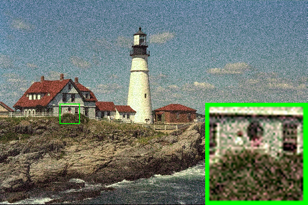
\includegraphics[width=1\textwidth]{comparea/resize_br_Noisy_nSig402030_kodim21.png}}
{\footnotesize (a) Noisy kodim21: 18.28dB }
\end{minipage}
\begin{minipage}[t]{0.195\textwidth}
\centering
\raisebox{-0.15cm}{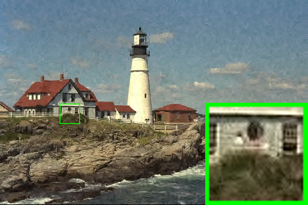
\includegraphics[width=1\textwidth]{comparea/resize_br_CBM3D_nSig402030_kodim21.png}}
{\footnotesize (b) CBM3D \cite{cbm3d}: 26.54dB}
\end{minipage}
\begin{minipage}[t]{0.195\textwidth}
\centering
\raisebox{-0.15cm}{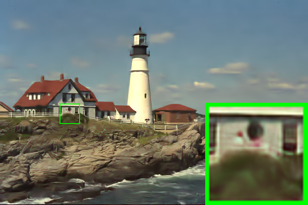
\includegraphics[width=1\textwidth]{comparea/resize_br_MLP_nSig402030_kodim21.png}}
{\footnotesize (c) MLP \cite{mlp}: 27.53dB}
\end{minipage}
\begin{minipage}[t]{0.195\textwidth}
\centering
\raisebox{-0.15cm}{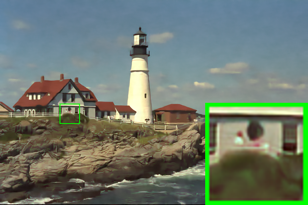
\includegraphics[width=1\textwidth]{comparea/resize_br_TNRD_nSig402030_kodim21.png}}
{\footnotesize (d) TNRD \cite{chen2015learning}: 27.60dB }
\end{minipage}
\centering
\begin{minipage}[t]{0.195\textwidth}
\raisebox{-0.15cm}{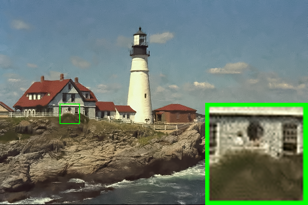
\includegraphics[width=1\textwidth]{comparea/resize_br_NC_nSig402030_kodim21.png}}
{\footnotesize (e) NC \cite{noiseclinic,ncwebsite}: 26.48dB  } 
\end{minipage}
}\vspace{-3mm}
\subfigure{
\begin{minipage}[t]{0.195\textwidth}
\centering
\raisebox{-0.15cm}{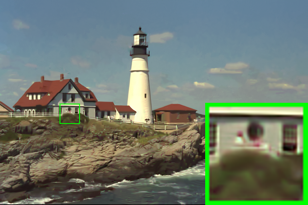
\includegraphics[width=1\textwidth]{comparea/resize_br_WNNMCW_nSig402030_kodim21.png}}
{\footnotesize (f) WNNM0: 27.80dB  }
\end{minipage}
\begin{minipage}[t]{0.195\textwidth}
\centering
\raisebox{-0.15cm}{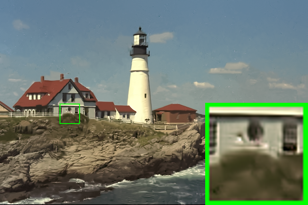
\includegraphics[width=1\textwidth]{comparea/resize_br_WNNMJ_nSig402030_kodim21.png}}
{\footnotesize (g) WNNM1: 27.75dB  }
\end{minipage}
\begin{minipage}[t]{0.195\textwidth}
\centering
\raisebox{-0.15cm}{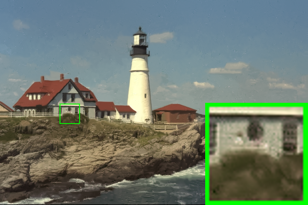
\includegraphics[width=1\textwidth]{comparea/resize_br_WNNM_ADMM_nSig402030_kodim21.png}}
{\footnotesize (h) WNNM2: 27.12dB }
\end{minipage}
\begin{minipage}[t]{0.195\textwidth}
\centering
\raisebox{-0.15cm}{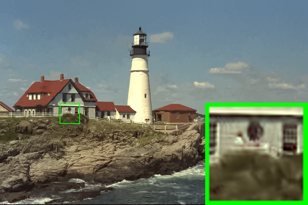
\includegraphics[width=1\textwidth]{comparea/resize_br_CWNNM_ADMM_nSig402030_kodim21.png}}
{\footnotesize (i) MC-WNNM: \textbf{28.34}dB}
\end{minipage}
\begin{minipage}[t]{0.195\textwidth}
\centering
\raisebox{-0.15cm}{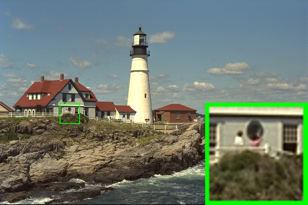
\includegraphics[width=1\textwidth]{comparea/resize_br_kodim21.png}}
{\footnotesize (j) Clean kodim21}
\end{minipage}
}\vspace{-0.5mm}
\caption{Denoised images of different methods on the image ``kodim21'' degraded by AWGN with different standard derivations of $\sigma_{r}=40, \sigma_{g}=20, \sigma_{b}=30$ on R, G, B channels, respectively. The images are better to be zoomed in on screen.}
\label{f3}
\vspace{-3mm}
\end{figure*}


{
\small
\bibliographystyle{unsrt}
\bibliography{egbib}
}

\end{document}